%!TEX root = ../../main.tex

% Processo de aprendizado OK
% Tarefa de classificação binária
% Divisão dos Dados
% Explicação do método holdout
% Parâmetros e hiperparâmetros
% Métricas Utilizadas - cenários balanceados e desbalanceados

A tarefa de aprendizado abordada neste trabalho consiste em uma tarefa de classificação binária. Neste contexto, uma imagem de $256 \times 256$ \emph{pixels} composta por duas assinaturas manuscritas, nas quais a primeira delas representa uma assinatura de referência genuína e a segunda compreende uma assinatura a ser verificada. A saída desejada é a predição da autenticidade da segunda assinatura e, por ser uma tarefa de classificação binária, só poderá possuir os valores de \emph{autêntica} ou \emph{forjada}, como mostrado na Figura \ref{fig:esquema-solucao}.

\begin{figure}[h!]
  \centering
  \caption{Uma visão geral do processo de aprendizado.}
  \label{fig:esquema-solucao}
  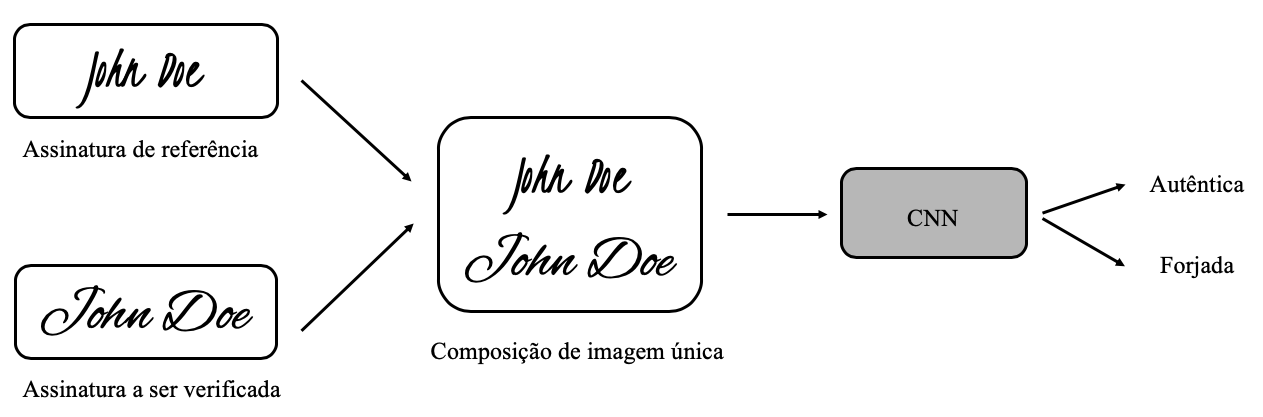
\includegraphics[width=\textwidth]{imgs/esquema-solucao}
\end{figure}

O treinamento e testes das CNNs seguirão o método \emph{holdout} de validação cruzada, em que $70\%$ dos dados serão utilizados no treino e ajuste de parâmetros, enquanto $20\%$ dos dados serão aproveitados para o processo de teste das redes, com vista a capturar o poder de generalização realizado pelos modelos considerados \cite{brink}. Os $10\%$ de dados restantes, serão utilizados para a validação do modelo durante o processo de treinamento.

Os modelos propostos serão avaliados perante as métricas de desempenho de \emph{Acurácia} e \emph{F-score}. A acurácia indica a porcentagem de predições corretas inferidas pelos modelos. O \emph{F-score}, por sua vez, é calculado pela média harmônica da precisão e da revocação
